\documentclass[a4paper]{iacas}

\usepackage{cite}
\usepackage{hyperref}% embedding hyperlinks [must be loaded after dropping]
\usepackage{amsmath,amsthm,amssymb,amsfonts,latexsym,mathrsfs,wasysym}
\usepackage{marvosym}
\usepackage{subcaption}
\usepackage{soul,color}
\usepackage{threeparttable}% tables with footnotes
\usepackage{dcolumn}% decimal-aligned tabular math columns
\usepackage{float}
\usepackage{graphicx}
\usepackage{accents}
\usepackage{tikz}
\usepackage{lastpage}
\usepackage{fancyhdr}
\usepackage{color}
\usepackage{cancel}
\usepackage{setspace}
%\doublespacing
% or:
\onehalfspacing
%\usepackage[T1]{fontenc}
%\usepackage{bigfoot} % to allow verbatim in footnote
\usepackage[framed,numbered]{matlab-prettifier}
\pagestyle{plain}
%\usepackage[hebrew,english]{babel}
\usetikzlibrary{shapes.geometric, arrows, calc}

\newcolumntype{d}{D{.}{.}{-1}}
\graphicspath{{figures/}}

% define some commands to maintain consistency
\newcommand{\pkg}[1]{\texttt{#1}}
\newcommand{\cls}[1]{\textsf{#1}}
\newcommand{\file}[1]{\texttt{#1}}
\newcommand{\sgn}[1]{\operatorname{sgn}\left(#1\right)}
\newcommand{\sat}[1]{\operatorname{sat}\left(#1\right)}
\newcommand{\rrule}[1]{\rule[#1]{0pt}{0pt}}
\newcommand{\fracds}[2]{\frac{\displaystyle #1\rrule{-0.2em}}{\displaystyle #2\rrule{1em}}}
\newcommand{\figref}[1]{Fig.~\ref{#1}}
\newcommand{\ubar}[1]{\underaccent{\bar}{#1}}
\newcommand{\norm}[1]{\lvert \lvert \vec #1 \rvert \rvert}

%diffeomorphism

\begin{document}


\begin{tabular}{l}
\\
{\bf\textit{Alexander Shender 328626114}} \\
{\bf\textit{Vladimir Tchuiev 309206795}} \\
Technion - Israel Institute of Technology
\end{tabular}

\vspace{2em}

\section{Optical Flow Section}

In Fig.~\ref{fig:100} we present the optical flow for $t=1$ and $N=16$. The red arrows represent the optical flow for a section of $16 \times 16$ pixels. It is evident that only the moving cars between frames have optical flow; while the footage is noisy, the eigenvalue limit for $A^T A$ allows to filter that noise, even in the expense of ignoring some moving parts.

\begin{figure}[!htbp]
	\centering
	\begin{subfigure}[b]{0.4\textwidth}
		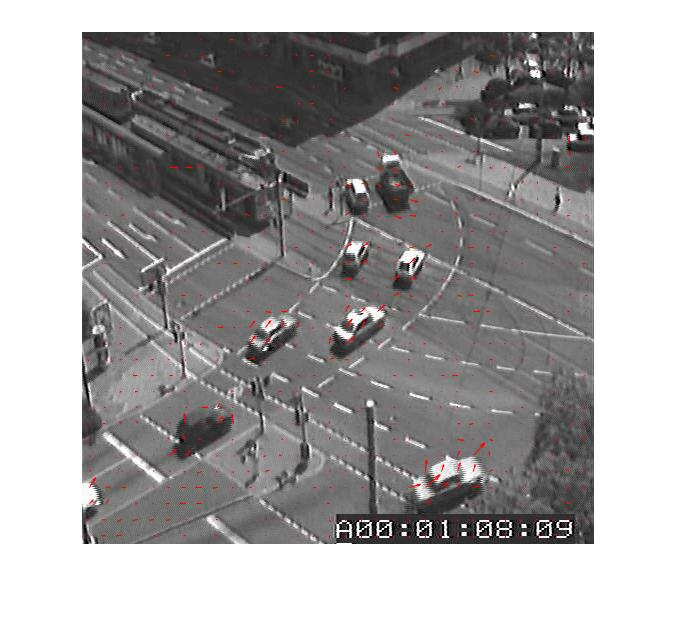
\includegraphics[width=\textwidth]{102.jpg}
		\caption{}
		\label{fig:102}
	\end{subfigure}
	%
	\begin{subfigure}[b]{0.4\textwidth}
		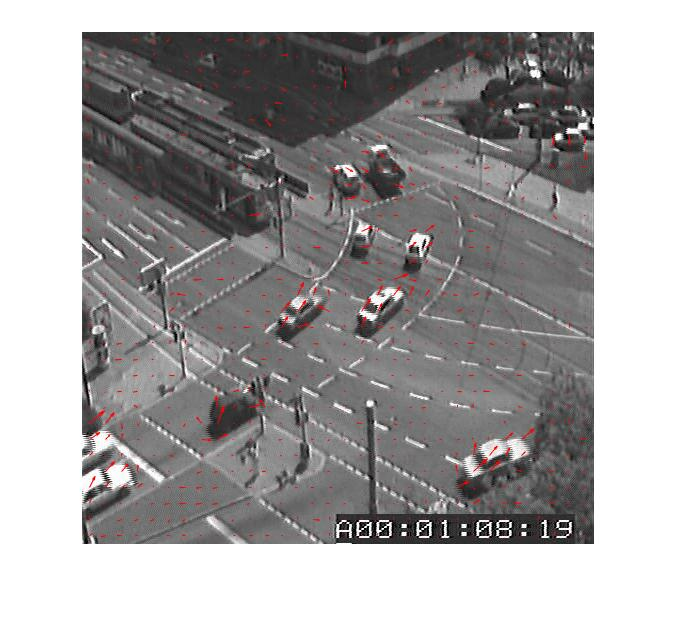
\includegraphics[width=\textwidth]{103.jpg}
		\caption{}
		\label{fig:103}
	\end{subfigure}

	\begin{subfigure}[b]{0.4\textwidth}
		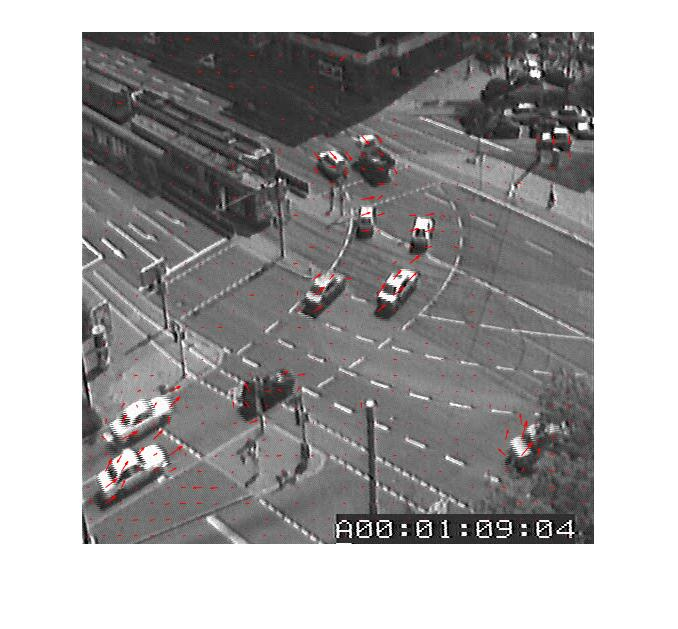
\includegraphics[width=\textwidth]{104.jpg}
		\caption{}
		\label{fig:104}
	\end{subfigure}
	%
	\begin{subfigure}[b]{0.4\textwidth}
		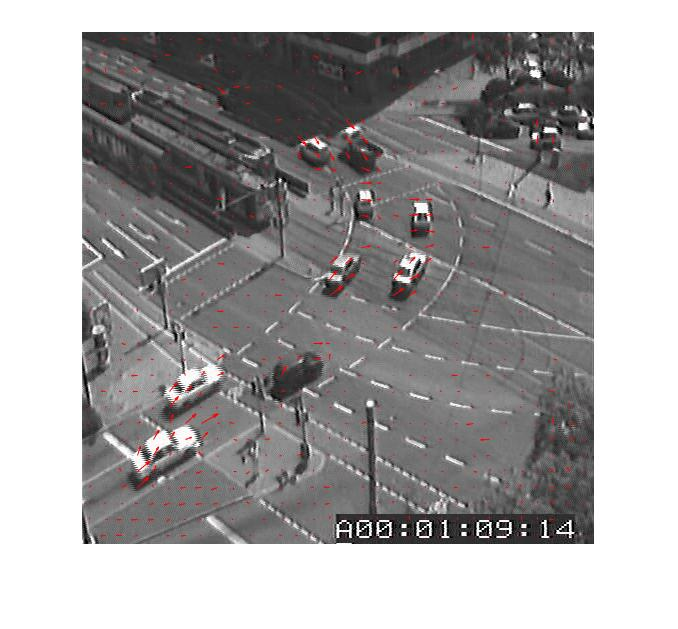
\includegraphics[width=\textwidth]{105.jpg}
		\caption{}
		\label{fig:105}
	\end{subfigure}

	\caption{Optical flow for frames $k=10, 20, 30,40$ with parameters $t=1$, $N=16$.}
	\label{fig:100}
\end{figure}

By lowering the eigenvalue lower limit to $t=0.1$ for Fig.~\ref{fig:300}, the optical flow is much more noisy and sensitive to the camera jitter, specifically note the roads in the figure.

\begin{figure}[!htbp]
	\centering
	\begin{subfigure}[b]{0.4\textwidth}
		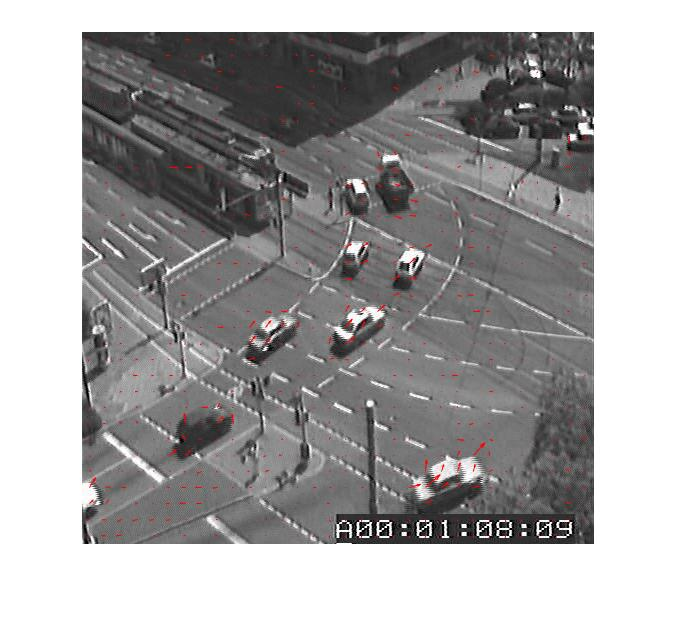
\includegraphics[width=\textwidth]{302.jpg}
		\caption{}
		\label{fig:302}
	\end{subfigure}
	%
	\begin{subfigure}[b]{0.4\textwidth}
		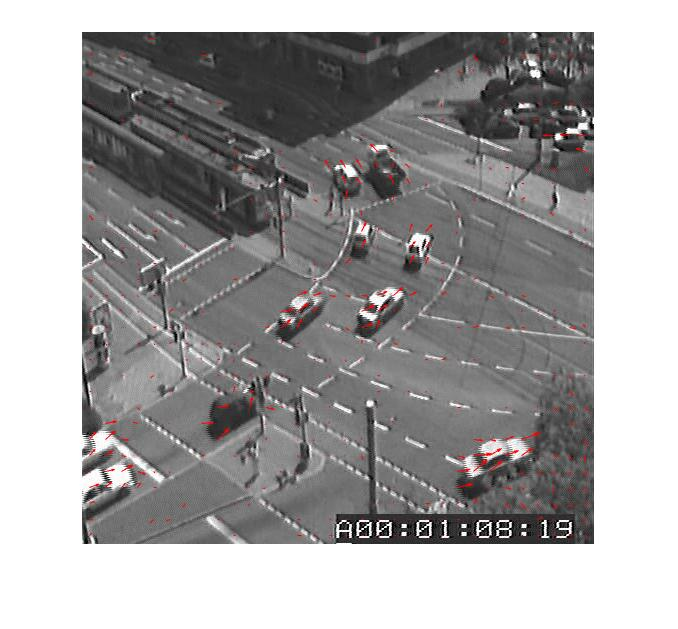
\includegraphics[width=\textwidth]{303.jpg}
		\caption{}
		\label{fig:303}
	\end{subfigure}
	
	\begin{subfigure}[b]{0.4\textwidth}
		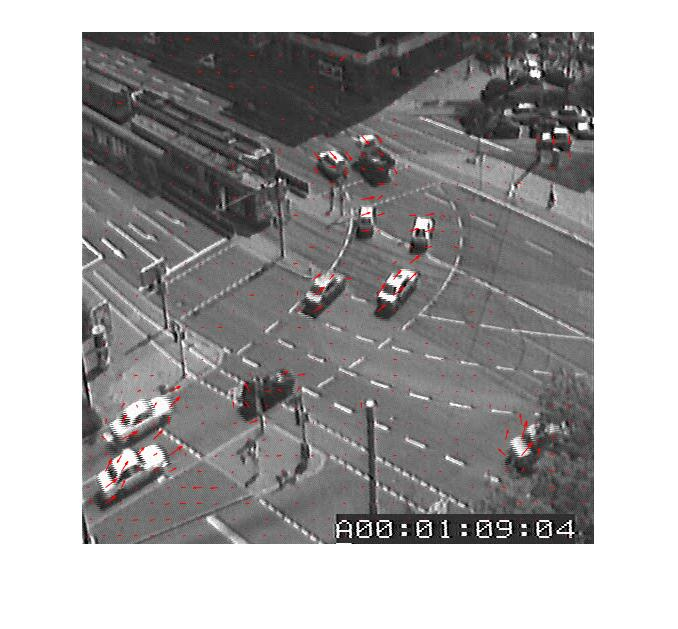
\includegraphics[width=\textwidth]{304.jpg}
		\caption{}
		\label{fig:304}
	\end{subfigure}
	%
	\begin{subfigure}[b]{0.4\textwidth}
		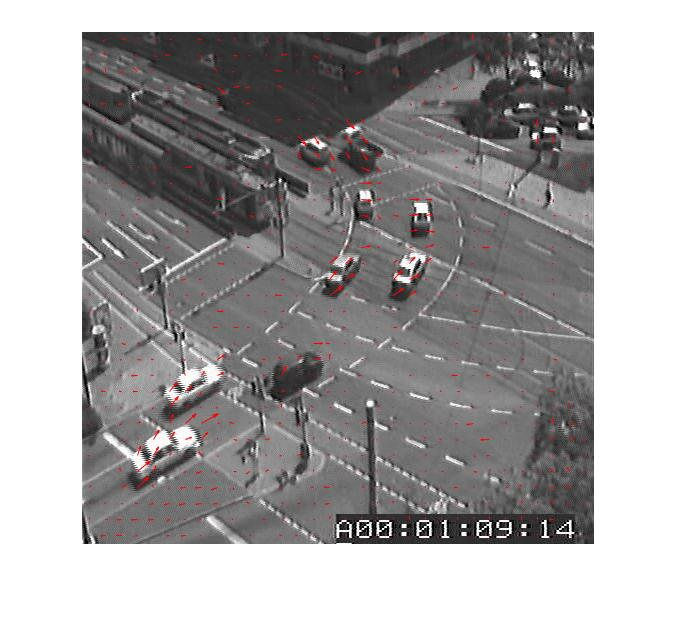
\includegraphics[width=\textwidth]{305.jpg}
		\caption{}
		\label{fig:305}
	\end{subfigure}
	
	\caption{Optical flow for frames $k=10, 20, 30,40$ with parameters $t=0.1$, $N=16$.}
	\label{fig:300}
\end{figure}

Setting the parameter $N=8$ increases the resolution of the optical flow segments, although with the cost of increased computational time and less data to work with per segment; increased resolution with optical flow requires a reduction in lower eigenvalue limit, as for smaller $A$ matrices the eigenvalue tend to be smaller as well. In Fig.~\ref{fig:400a} the optical flow is filtered out, even legitimate sections with moving parts while in Fig.~\ref{fig:400b} the optical flow shows similar results to Fig.~\ref{fig:100} although with higher resolution.

\begin{figure}[!htbp]
	\centering
	\begin{subfigure}[b]{0.4\textwidth}
		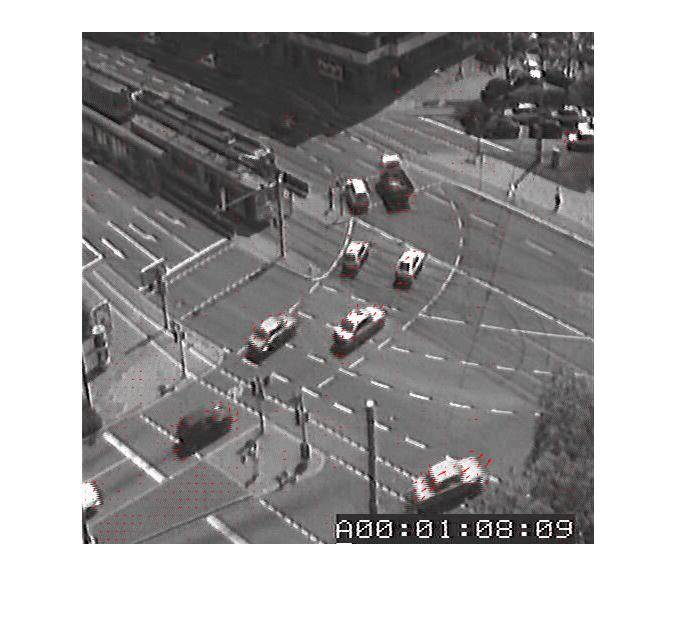
\includegraphics[width=\textwidth]{402.jpg}
		\caption{}
		\label{fig:402}
	\end{subfigure}
	%
	\begin{subfigure}[b]{0.4\textwidth}
		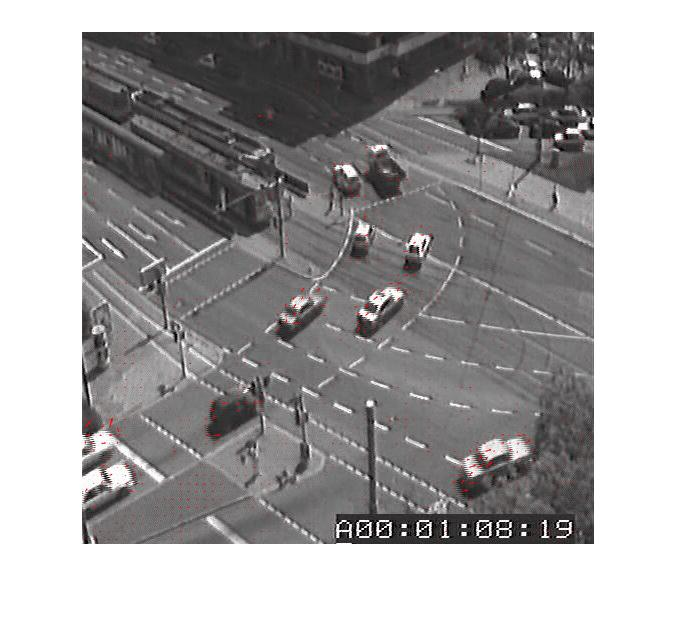
\includegraphics[width=\textwidth]{403.jpg}
		\caption{}
		\label{fig:403}
	\end{subfigure}
	
	\begin{subfigure}[b]{0.4\textwidth}
		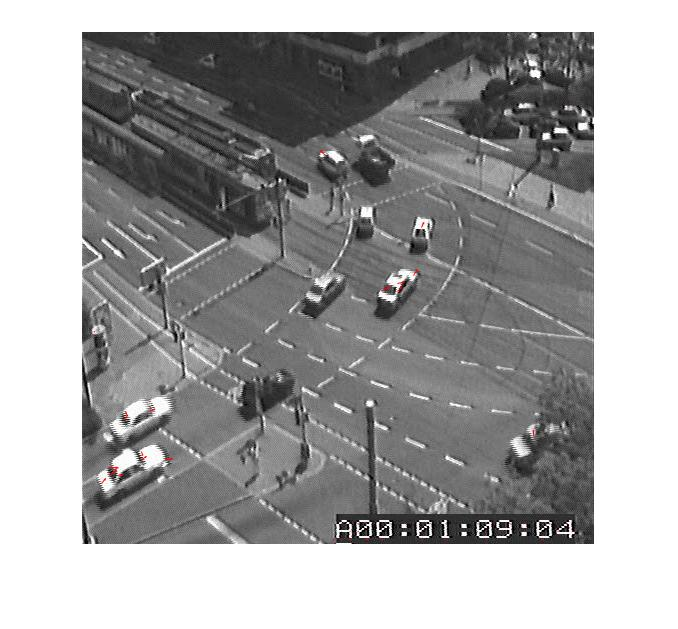
\includegraphics[width=\textwidth]{404.jpg}
		\caption{}
		\label{fig:404}
	\end{subfigure}
	%
	\begin{subfigure}[b]{0.4\textwidth}
		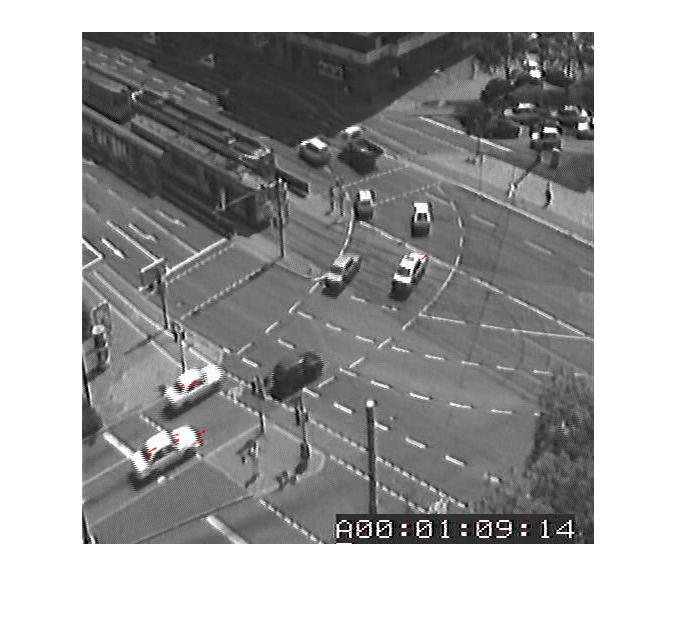
\includegraphics[width=\textwidth]{405.jpg}
		\caption{}
		\label{fig:405}
	\end{subfigure}
	
	\caption{Optical flow for frames $k=10, 20, 30,40$ with parameters $t=1$, $N=8$.}
	\label{fig:400a}
\end{figure}

\begin{figure}[!htbp]
	
	\centering
	\begin{subfigure}[b]{0.4\textwidth}
		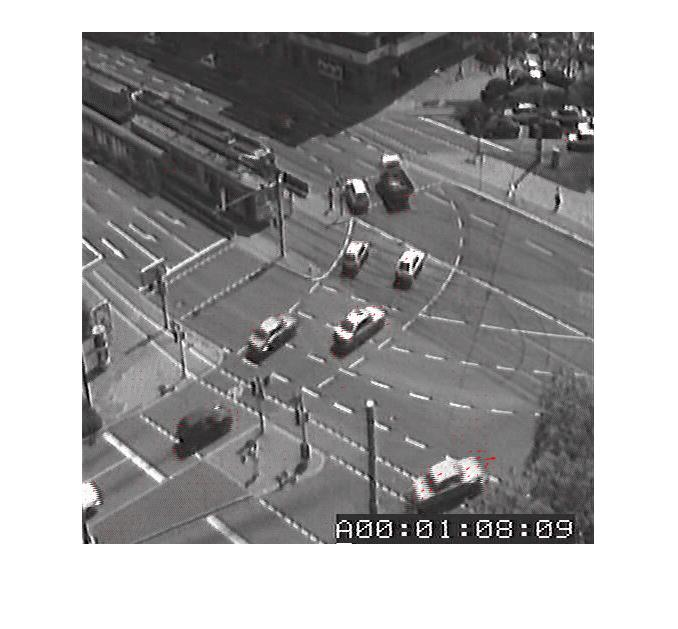
\includegraphics[width=\textwidth]{407.jpg}
		\caption{}
		\label{fig:407}
	\end{subfigure}
	%
	\begin{subfigure}[b]{0.4\textwidth}
		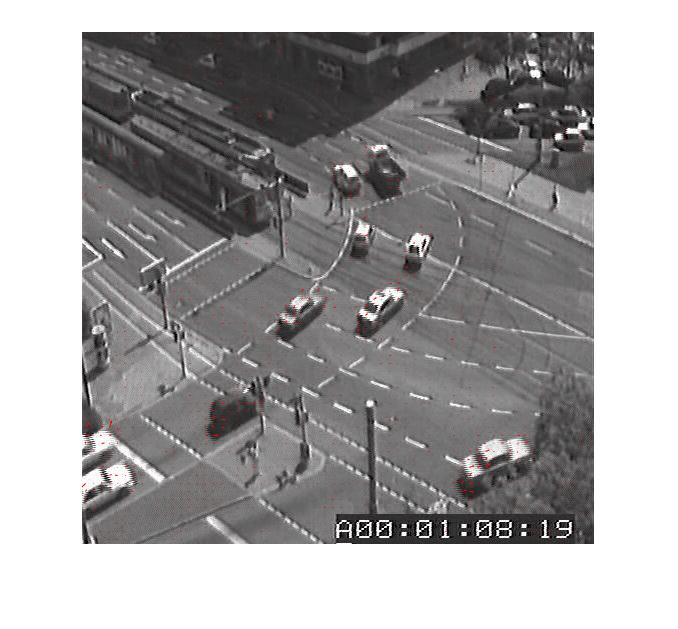
\includegraphics[width=\textwidth]{408.jpg}
		\caption{}
		\label{fig:408}
	\end{subfigure}
	
	\begin{subfigure}[b]{0.4\textwidth}
		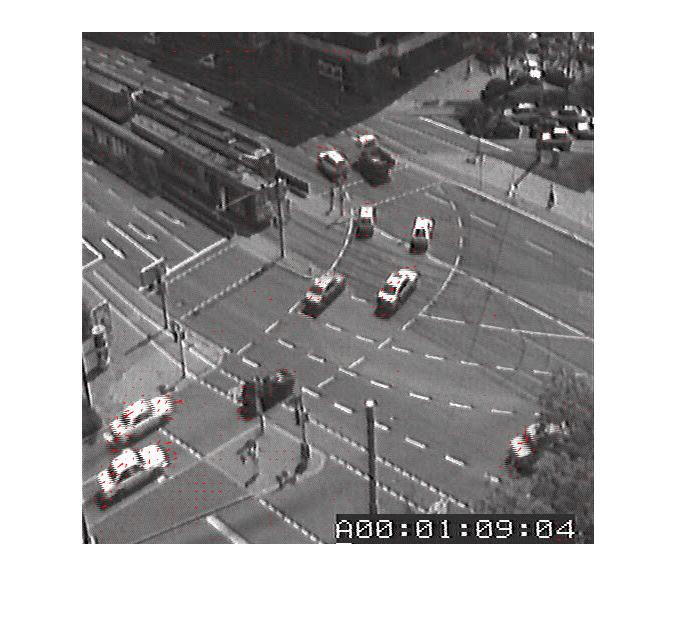
\includegraphics[width=\textwidth]{409.jpg}
		\caption{}
		\label{fig:409}
	\end{subfigure}
	%
	\begin{subfigure}[b]{0.4\textwidth}
		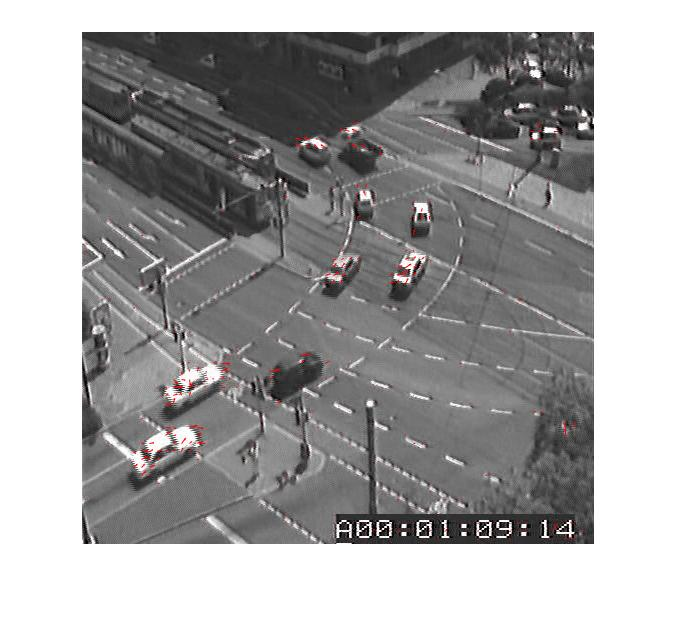
\includegraphics[width=\textwidth]{410.jpg}
		\caption{}
		\label{fig:410}
	\end{subfigure}
	
	\caption{Optical flow for frames $k=10, 20, 30,40$ with parameters $t=0.1$, $N=8$.}
	\label{fig:400b}
\end{figure}

\end{document}




